\documentclass[a4paper, 11pt]{article}
\usepackage{comment} % enables the use of multi-line comments (\ifx \fi) 
\usepackage{lipsum} %This package just generates Lorem Ipsum filler text. 
\usepackage{fullpage} % changes the margin
\usepackage{hyperref}
\usepackage{graphicx}

\begin{document}
%Header-Make sure you update this information!!!!
\noindent
\large\textbf{Assignment 4} \hfill \textbf{Tyler Wilding} \\
\normalsize COSC 2596 \hfill Due Date: 04/11/16 \\
Dr. Miguel Garcia-Ruiz \hfill \\
TA: -- \hfill

\section*{Brief Description of App}
The app I choose is a news app \href{https://play.google.com/store/apps/details?id=com.manoramaonline.mmtv}{Manorama News}.  It is a very cluttered and visually displeasing app that has quite a handful of negative reviews, and as a result it is a useful case study for this assignment.

\section*{Screenshots of App} 
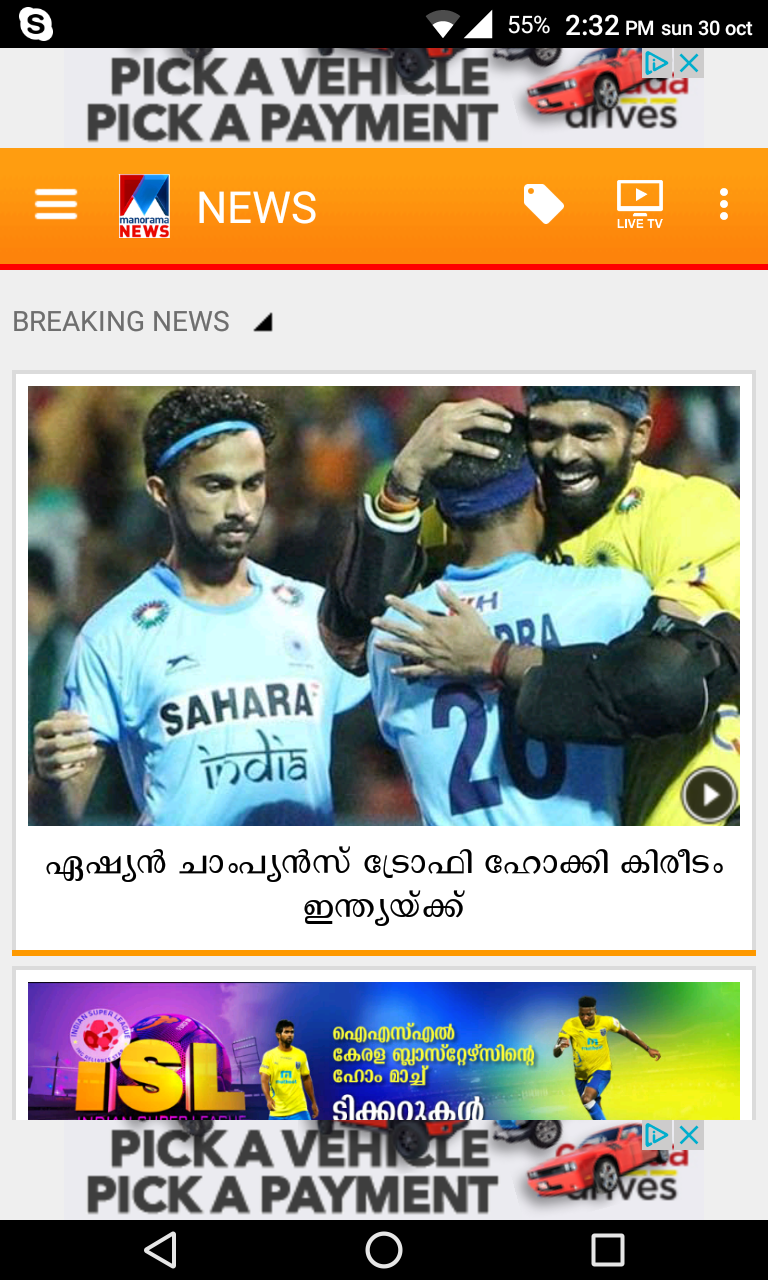
\includegraphics[scale=0.15]{sa.png}
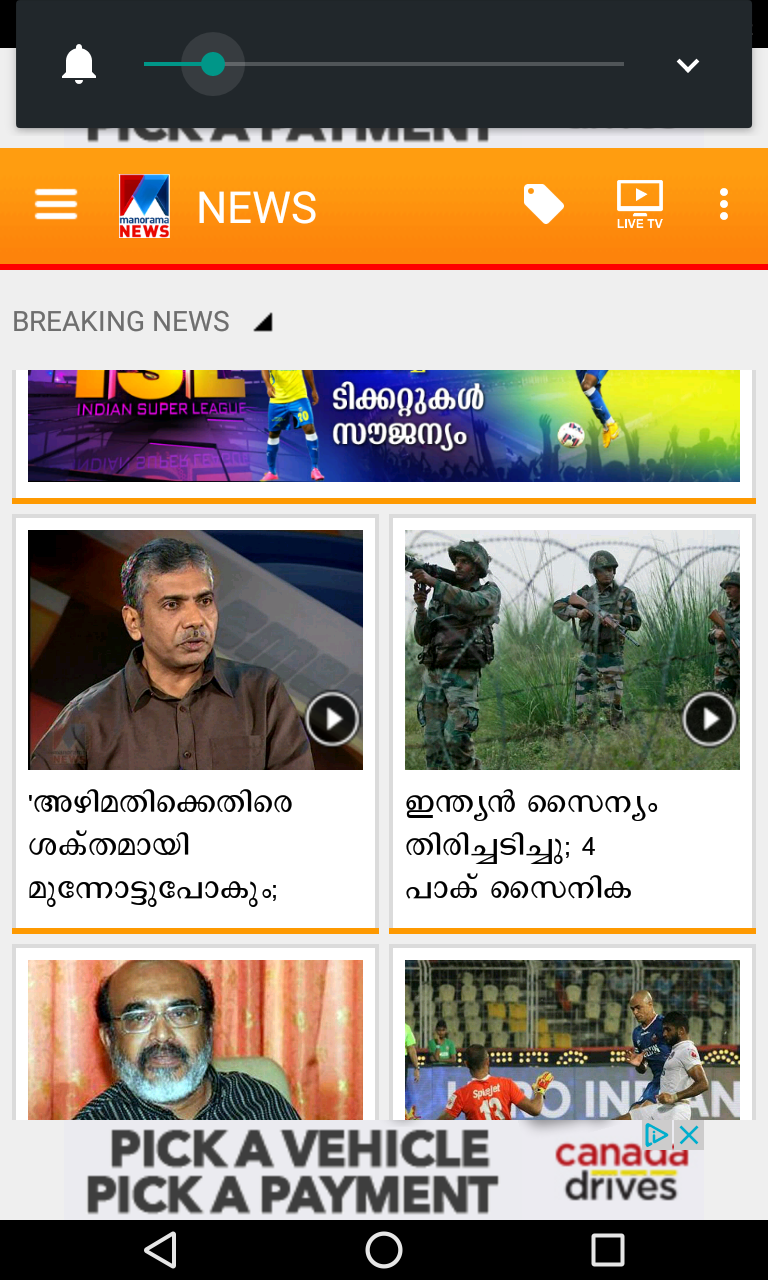
\includegraphics[scale=0.15]{sb.png}
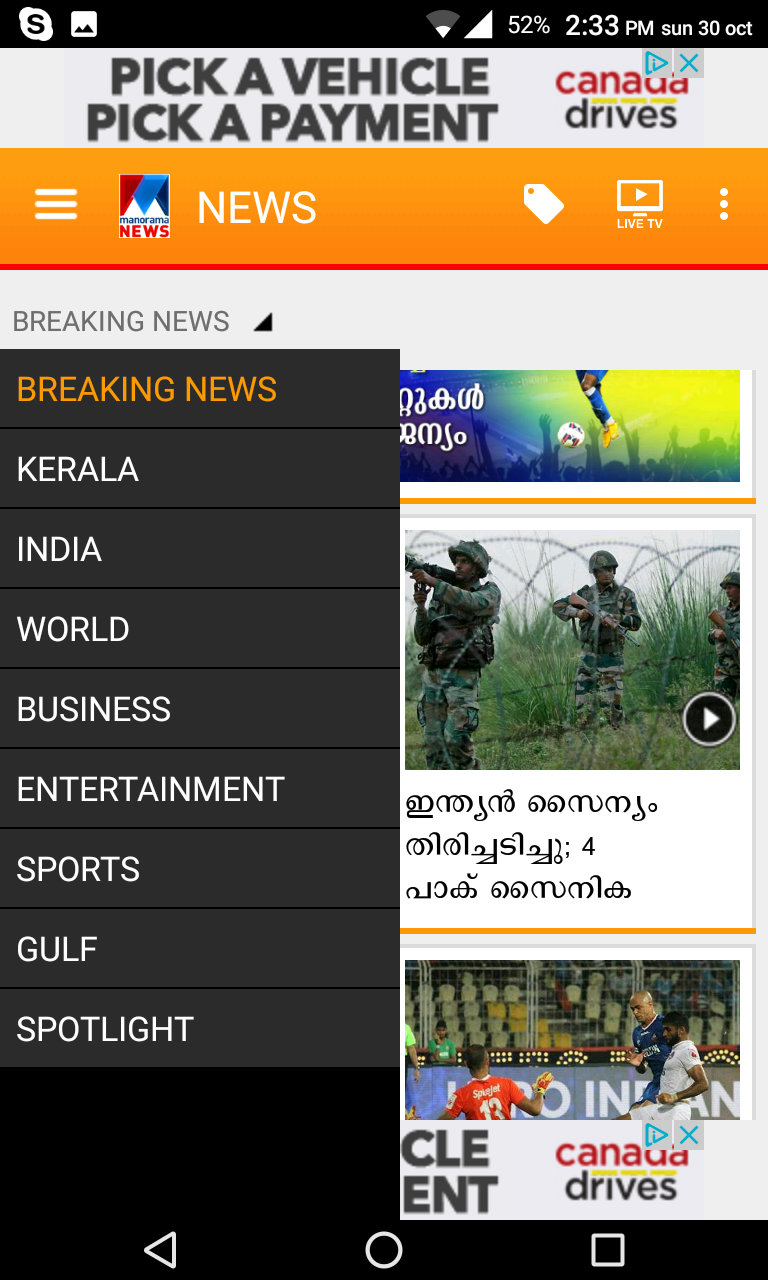
\includegraphics[scale=0.15]{sc.png}
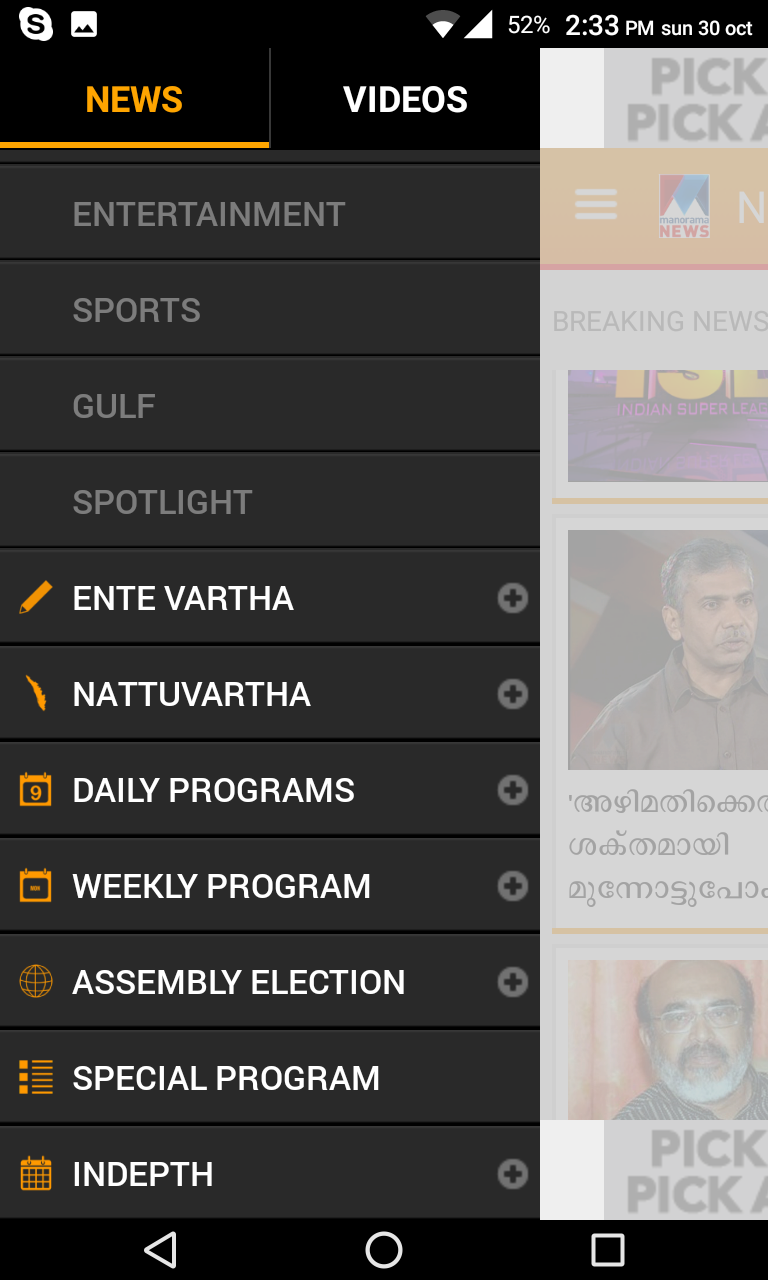
\includegraphics[scale=0.15]{sd.png}
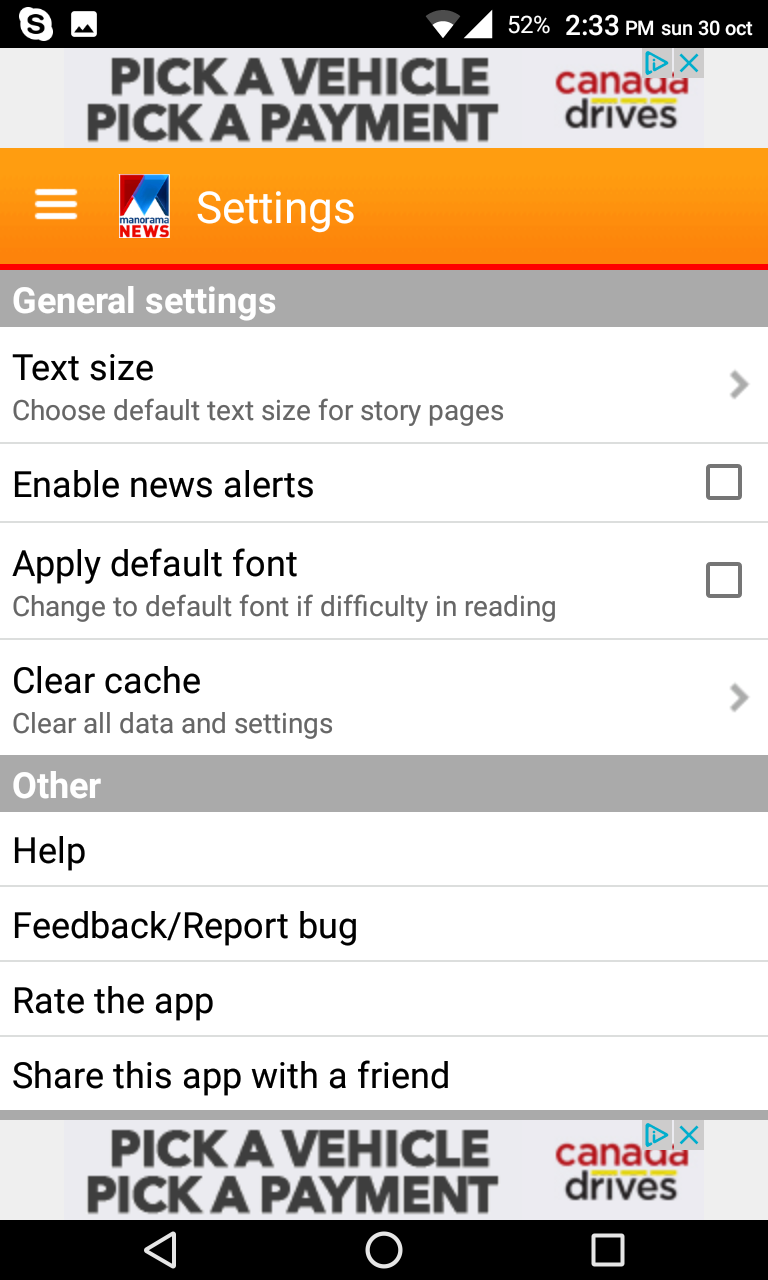
\includegraphics[scale=0.15]{se.png}
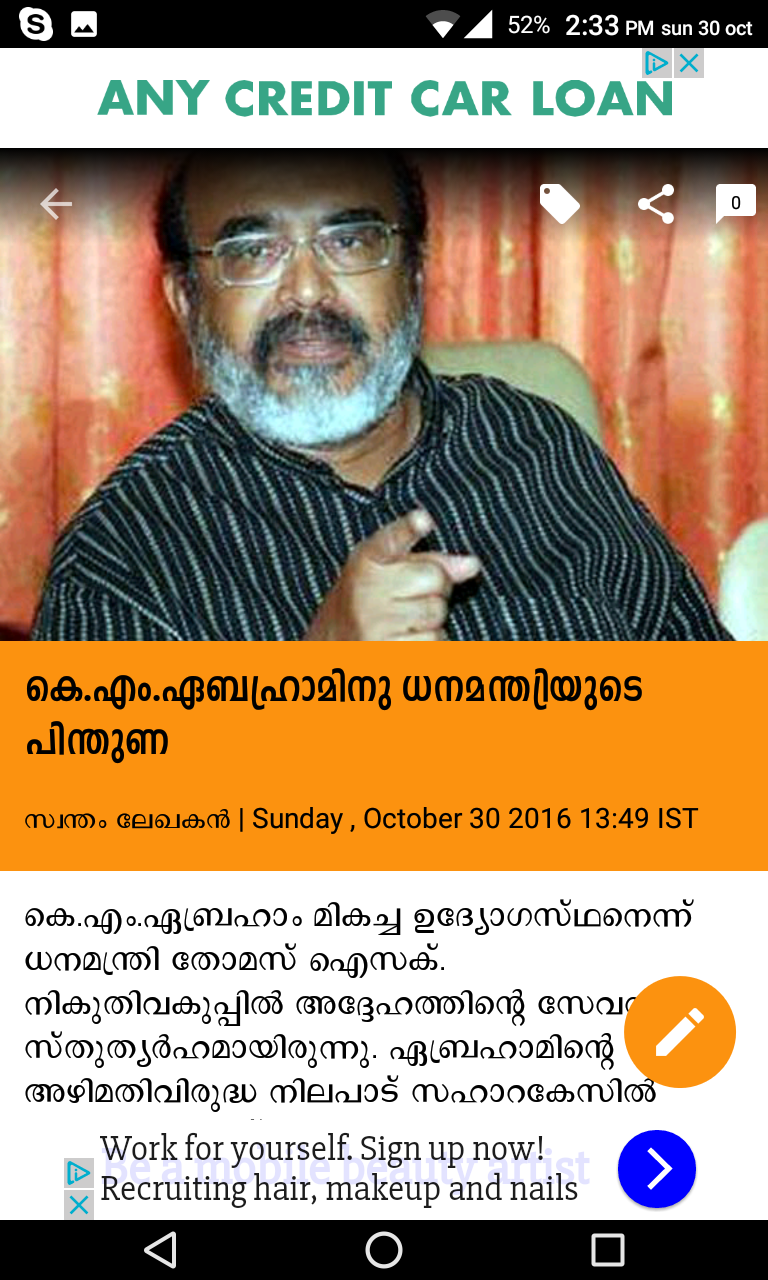
\includegraphics[scale=0.15]{sf.png}
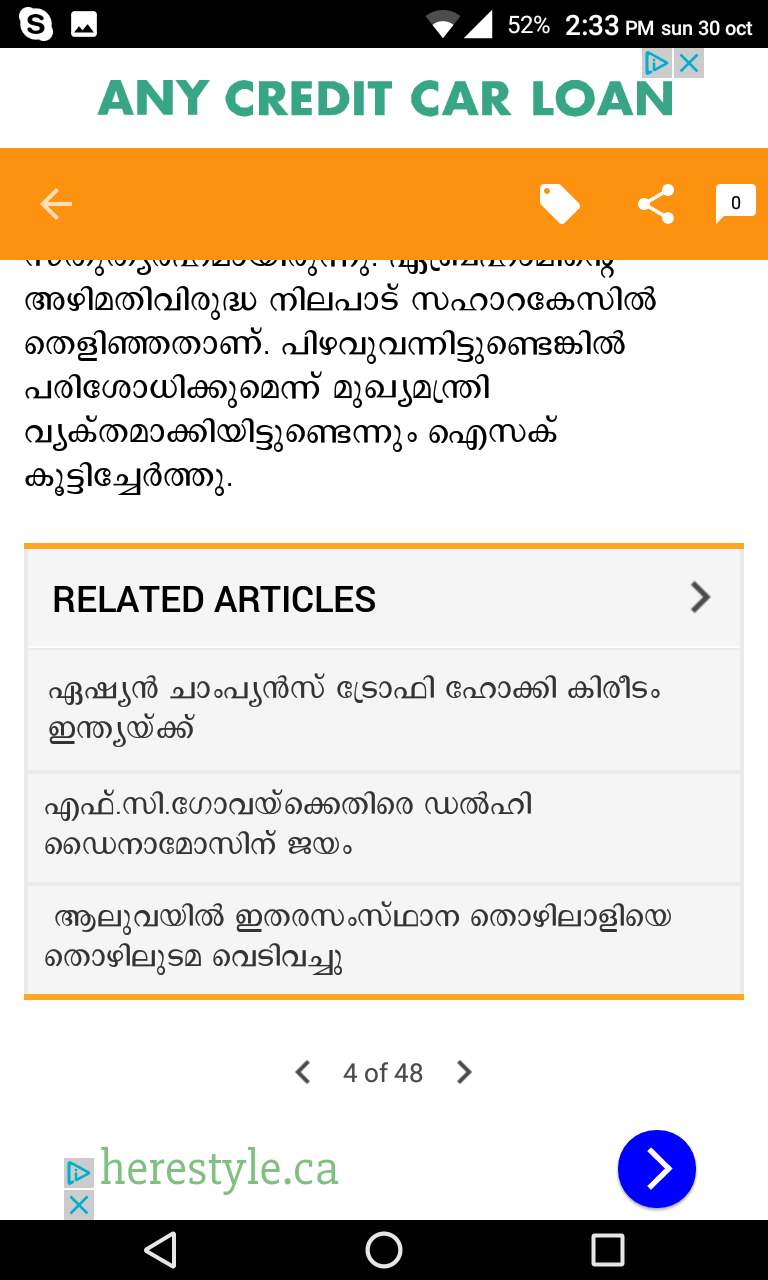
\includegraphics[scale=0.15]{sg.png}


\section*{Sketch}
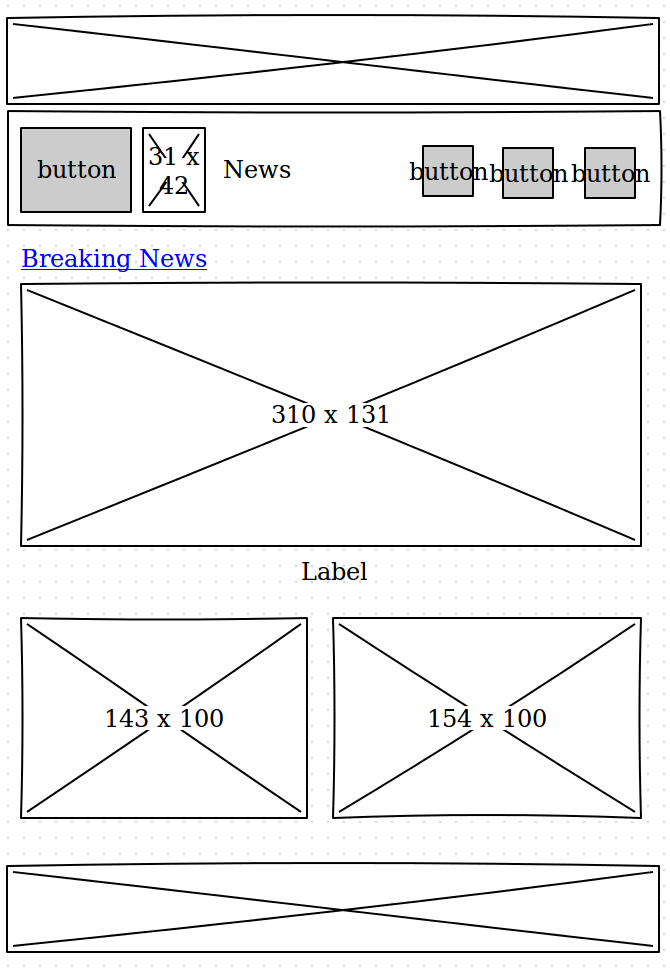
\includegraphics[scale=0.25]{sketch.png}

\section*{Suggested Improvements on Current Design}
Looking at the sketch that was produced for the main homepage of the app, we can see many problems.  First off, a quarter of the screen (top and bottom combined) are used for just ad space.  This clutters the presentation of the content and distracts because they are animated apps as well.  In addition, there is very little content to look at on the homepage, images are extremely large and sometimes you cannot even see the titles without scrolling down immediately.\\

My suggestions would be to remove the obtrusive ads as to make it much more visually appleasing.  I would also change the layout of the articles and sizes of the images to follow the Card design pattern more closely.  I would also remove the news dropdown menu on the topleft as this can already be accessed by swiping to the right to open the main menu.  This main menu as well could take up less of the screen in an effort to still see some of the content.  Some of the buttons and navigational elements of the app are very small and hard to touch as well.  Additionally, you can even see on the main article page how simplistic and visually unappealing it is, the image is still extremely large, and the text is bland with a total lack of color and emphasis on the page.  Overall, the app feels very cramped and displeasing.

\section*{Low Fidelity Prototype}
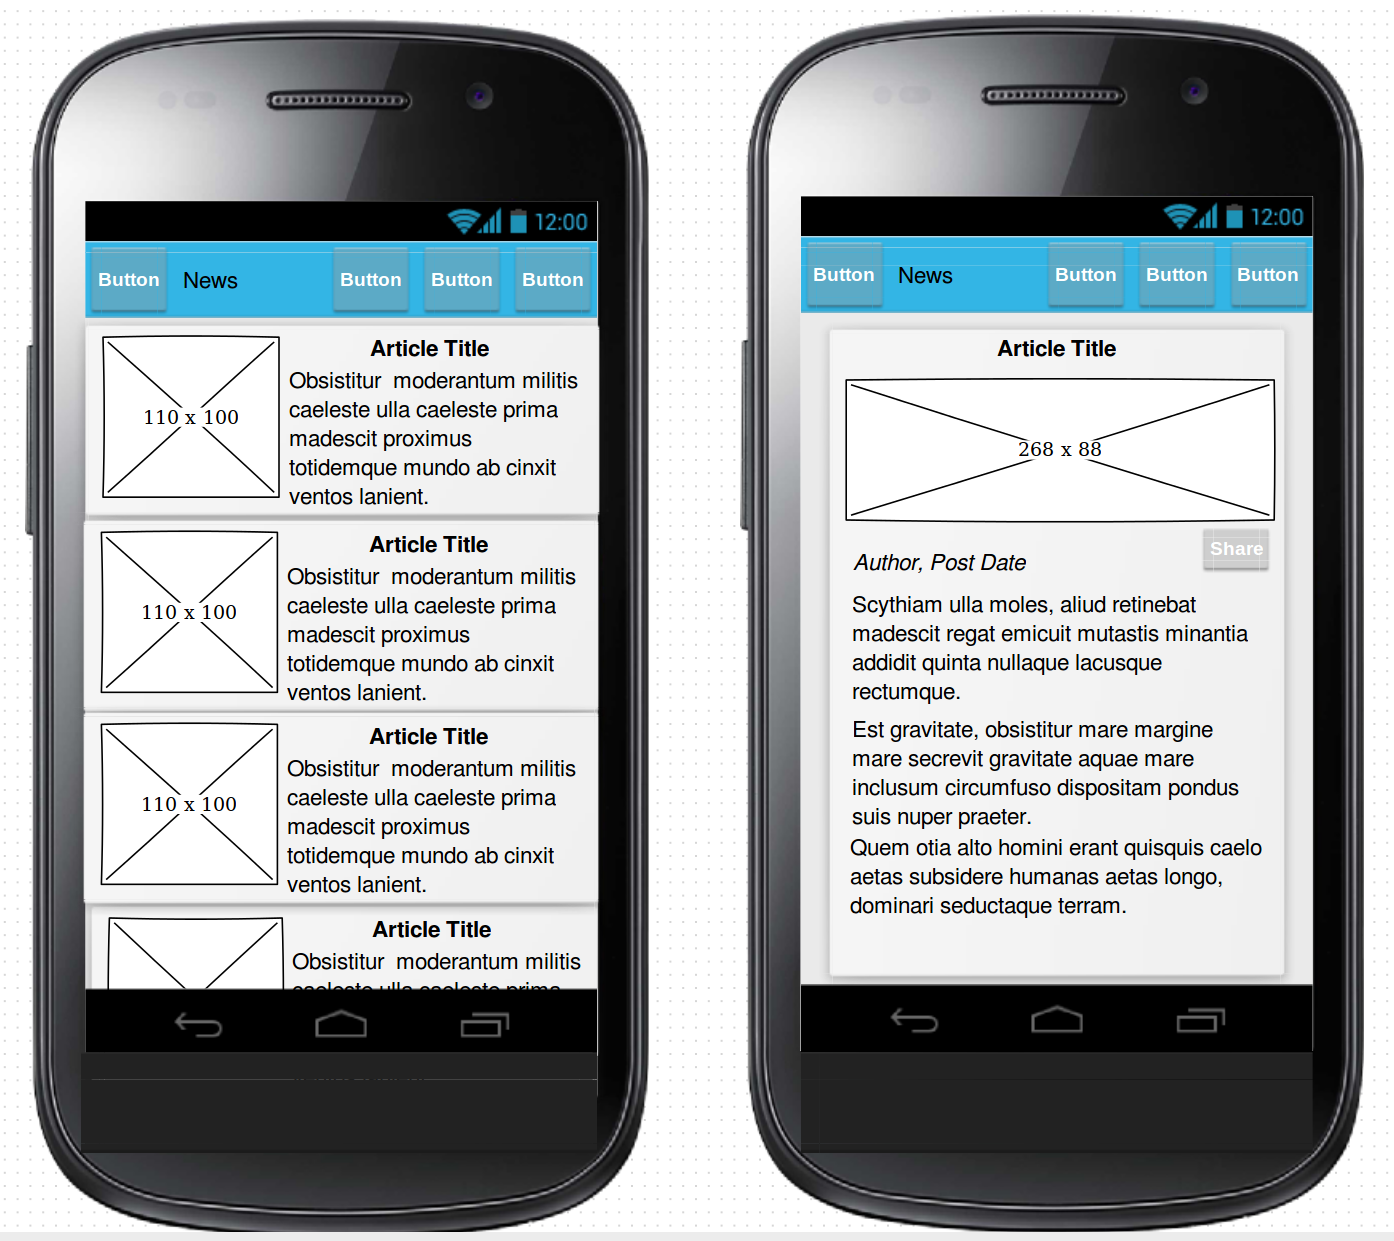
\includegraphics[scale=0.25]{lowfi.png}

\section*{How were Cooper's Guidelines Utilized}
\subsection*{Don't think of your product as a computer}
This idea is taken into account because the design has been improved to be more user friendly on a touch-screen device.  This means that the inputs and controls are now actually usable and noticable.  It also more obviously supports scrolling and paradigms that other mobile phone applications use that users are already familiar with.  Phones are also often used as a social device as well, adding share buttons supports this trend.

\subsection*{Integrate hardware and software design}
A holistic experience is produced with this design as the software and therefore the design of the app integrates well with the hardware features of the phone. By supporting touch and making it simplistic to use again, the touchscreen feels intuitive and meant to be used.  Likewise, using the phones built-in WiFi to share articles and to read more articles is the principle feature of the application.

\subsection*{Let context drive design}
This application will be used to read news articles, that is the main purpose from the beginning.  The old design was distracting from this with ads, and a layout that did not tell you very much about the article you were about to read.  With the new design, it fully supports the needs and wants of the intended-user.  Users can easily see a quick summary of the articles and decide if they want to read further, instead of just a crafted headline to draw a users attention. 

\subsection*{Use modes judiciously, if at all}
There are not many modes for this application, the old app supported a video feature, however that is not shown in the low-fidelity prototypes and in my opinion should not be included in this app at all, because it distracts from the main purpose.  If an article itself had an embedded video that would be fine, but having a seperate page just to watch videos is not a good idea.

\subsection*{Limit the Scope}
As we have mentioned in the previous points, the app is now limited on what it can do, but this is a good thing.  Users download a news app to read about the news, not watch ads or videos.  As a result, by focusing on what users will actually be using the app for the design can also be focused on what the user is looking for and the content can be presented immediately.

\subsection*{Balance navigation with display density}
This is the largest improvement from the old design where the app was cluttered and almost to the point of un-usable.  Now with the new design, more information is displayed in a relatively compact fashion while also improving navigation with simple scrolling and clicking.  The screen space on a phone is always limited so wasting it with ad space is a great way to drive away potential users.

\subsection*{Minimize input complexity}
There are not many forms of input for the application, only simply button touches and scrolling, exactly what a typical mobile phone user would come to expect and it should be easy for them to pick up and use.

\section*{Design Pattern Discussion}
This design pattern follows the Cards design paradigm, which is been heavily pushed by Google's design team for the use especially in mobile phones.  This is because touch is a more intuitive form of input and as a result, having a design pattern that better represents the real world and how objects interact is the best way to make the user interfaces and user experiences more pleasant.  Among other principles, the idea behind Cards is to have distinct pieces of information that can be scrolled, manipulated, and interacted with.  When used in a layout such as this, the interface resembles a stack of cards and the user cycles through them to find the one they are looking for.  However, often times the Cards design pattern is overused and creates a lot of empty wasted space between the cards.  While some may argue this makes the interface more easier to see and this is true, it should not be used for content that only differs slightly such as the article names and descriptions.  In this scenario, as showcase in the low-fidelity prototype, you want the cards to be close together, therefore maximizing screen real-estate.\\

There is much more details and guidelines proposed by the Google material design page that covers everything for how things should more naturally be animated and how to stress emphasis in certain aspects to draw the users attention, but these are very difficult to represent on a low-fidelity prototype.  The main thing from the design pattern that people associate is the very simplistic and flat look, and how certain elements stand out from the rest to immediately help users understand the affordances of the application.\\

More information about Google Material can be found \href{https://material.google.com/#introduction-principles}{here} and about the design pattern of cards specifically, \href{https://material.google.com/components/cards.html}{here}

\end{document}
